\section*{M05 — Symbolic Collapse and Reconfiguration: Diagnostic Vectors and Clinical Translation}

This module operationalizes the symbolic triad $(\alpha, \kappa, \mathcal{E}_r)$ in diagnostic and translational contexts. Building on the geometric formalism from M04, we simulate trajectories through cognitive phase space and model symbolic breakdown and reorganization as computable processes. We present clinical scenarios, propose symbolic biomarkers, and articulate a translational framework for epistemic diagnostics.

\subsection*{5.1 Clinical Phase Diagrams and Symbolic Trajectories}

We introduce a symbolic phase space defined by the triad $(\alpha, \kappa, \mathcal{E}_r)$, in which cognitive dynamics unfold as vector trajectories modulated by entropy, curvature, and anchoring. Each point in this three-dimensional space represents a symbolic-cognitive state, while the direction and magnitude of movement reflect its recursive evolution. This framework allows us to visualize and simulate both collapse trajectories and recovery arcs in formal, topological terms.

The $\alpha$ axis represents epistemic anchoring—the system's ability to maintain coherent narrative self-referential stability. The $\kappa$ axis denotes symbolic curvature—how densely symbolic associations are packed or folded in meaning space. The $\mathcal{E}_r$ axis models recursive entropy—the proliferation of unresolved symbolic recursion or semantic uncertainty over time.

Clinical states correspond to trajectories within this manifold:

\begin{itemize}
  \item \textbf{Stability basin:} regions where $\alpha$ is high, $\kappa$ is moderate, and $\mathcal{E}_r$ remains bounded.
  \item \textbf{Pre-collapse zone:} $\alpha$ begins to decrease while $\kappa$ and $\mathcal{E}_r$ rise, indicating semantic overload.
  \item \textbf{Collapse attractors:} critical zones where $\mathcal{E}_r$ diverges, $\alpha \to 0$, and symbolic implosion or explosion occurs.
  \item \textbf{Recovery basin:} phase-space regions where entropy decreases and anchoring is reestablished.
\end{itemize}

We define a symbolic trajectory as a continuous function:

\[
\gamma(t) = (\alpha(t), \kappa(t), \mathcal{E}_r(t))
\]

where $t$ is symbolic or phenomenological time. Using simulated dynamics, we can trace $\gamma(t)$ across the phase manifold to identify risk periods, collapse inflection points, and optimal paths for recovery steering.

The next sections instantiate these ideas through anchoring vector fields, simulated archetypes, and reconfiguration modeling.
\subsection*{5.2 Anchoring Vectors and Collapse Forecasting}

To navigate collapse and recovery within the symbolic manifold, we introduce the concept of anchoring vectors—gradients that model the directionality of epistemic stabilization or destabilization in $(\alpha, \kappa, \mathcal{E}_r)$ space. These vectors represent the cognitive system's spontaneous or assisted trajectory under symbolic tension.

The dynamics of symbolic collapse can be formalized as a flow field:

\[
\vec{v}_{\text{collapse}} = \nabla \mathcal{E}_r - \lambda \nabla \alpha
\]

and its complementary recovery vector field:

\[
\vec{v}_{\text{recovery}} = -\nabla \mathcal{E}_r + \lambda \nabla \alpha
\]

where $\lambda$ is a subject-specific resilience coefficient, modulating the weight of anchoring over entropy gradients. This formulation allows us to simulate both pathological drift and recovery arcs in the same phase space.

Clinically, the anticipation of symbolic rupture may become feasible by tracking the velocity and divergence of $\vec{v}(t)$. For instance, zones of high $\nabla \mathcal{E}_r$ with vanishing $\nabla \alpha$ suggest pre-collapse turbulence. Analogously, recovery is marked by trajectories with converging $\vec{v}_{\text{recovery}}$ vectors toward epistemic attractors.

We propose that symbolic forecasting tools—based on natural language entropy, speech coherence (Mota et al., 2017\cite{Mota2017}), and curvature metrics—could be trained to recognize such divergences. These indicators may serve as early warning signals of collapse, or guidance vectors for therapeutic intervention.

As a concrete example, consider an individual whose symbolic narrative begins to fragment, reflected in increasing semantic dispersion and decreasing referential cohesion. In such a case, entropy metrics would rise while anchoring would decay—projecting a trajectory directed toward a collapse basin. A vectorial analysis of the subject’s $\vec{v}(t)$ could then suggest symbolic steering—therapeutic reframing, narrative reinforcement, or memory reconsolidation—to reroute the trajectory.

This dynamical approach reframes psychiatric monitoring as phase-space navigation: the goal is not to suppress symptoms but to realign symbolic flow within a region of semiotic stability and epistemic coherence.
\subsection*{5.3 Simulated Patient Archetypes}

To concretize the symbolic manifold model, we now describe four simulated archetypes that illustrate distinct trajectories of symbolic collapse and potential recovery. Each archetype traces a characteristic path $\gamma(t)$ within the phase space defined by $(\alpha, \kappa, \mathcal{E}_r)$, representing different neurocognitive and epistemic configurations.

\textbf{1. The Visionary Disintegrant} \\
This subject begins in a state of high curvature ($\kappa$), moderate anchoring ($\alpha$), and low entropy ($\mathcal{E}_r$). A phase of overassociation unfolds—symbolic density increases without proportional anchoring, leading to torsion and implosion. Clinically, this may resemble hypomanic or delusional creativity. Without intervention, anchoring collapses and entropy rises, culminating in a semantic breakdown. Recovery requires restoring referential stability while preserving creative curvature.

\textbf{2. The Saturated Mind} \\
Initially exhibiting high $\alpha$ and high $\kappa$, this archetype encounters sustained information overload. As $\mathcal{E}_r$ grows, the system enters a pre-collapse spiral, marked by recursive loops of unresolved symbols. This manifests as obsessive ideation or derealization. Intervention must target entropy discharge—via expressive or symbolic processing—and modulation of curvature density.

\textbf{3. The Epistemic Survivor} \\
Following a deep collapse ($\alpha \approx 0$, $\mathcal{E}_r \gg 1$), this subject shows spontaneous re-emergence of anchoring through symbolic pattern recognition or external narrative scaffolding (e.g., therapeutic dialogue). The recovery vector is steered by a sudden gradient in $\nabla \alpha$ due to contextual reanchoring. This archetype validates the reversibility of collapse via narrative restitution.

\textbf{4. The Creative Singularity} \\
A rare archetype characterized by stable oscillations in $\kappa$ and bounded $\mathcal{E}_r$, despite low $\alpha$. This configuration may reflect states of altered consciousness, mystical insight, or high-functioning giftedness. Instead of collapse, symbolic structures fluctuate around a stable strange attractor. Interventions here may aim not at normalization but at facilitating meaningful integration.

These archetypes serve as symbolic-dynamic templates, enabling future simulations and diagnostic topologies. They also reflect the hypothesis that not all departures from normative anchoring are pathological—some may reflect transitions toward new symbolic configurations that demand epistemic expansion, not suppression.

\subsection*{5.4 Recovery Dynamics and Epistemic Reintegration}

Recovery from symbolic collapse is not a simple return to baseline. It is a dynamic process of epistemic reintegration that unfolds across multiple axes—narrative, affective, semantic, and structural. Within our manifold $(\alpha, \kappa, \mathcal{E}_r)$, recovery is marked by the reversal of entropy gradients, the reconstitution of anchoring, and the recalibration of symbolic curvature.

The trajectory $\gamma(t)$ of a recovering subject typically involves three distinguishable phases:

\begin{enumerate}
  \item \textbf{Entropy attenuation:} a deceleration in $\mathcal{E}_r$ growth, often catalyzed by expressive processing, containment, or therapeutic resonance. Symbolic recursion becomes bounded again.
  \item \textbf{Anchoring reactivation:} a spontaneous or guided increase in $\alpha(t)$, representing re-engagement with narrative structures, autobiographical memory, or intersubjective validation.
  \item \textbf{Curvature modulation:} the fine-tuning of $\kappa$ to achieve symbolic complexity without fragmentation—high enough for generativity, low enough for coherence.
\end{enumerate}

Epistemic reintegration occurs when the symbolic system stabilizes within a bounded region of phase space—a new attractor of meaning. In clinical terms, this may manifest as narrative restitution, coherent re-signification of past trauma, or restoration of dialogical self-structure. The goal is not merely the absence of symptoms, but the emergence of a reorganized symbolic topology that supports sustainable self-reference.

Importantly, recovery may produce novel configurations not isomorphic to the pre-collapse state. As such, interventions should not aim at restoring a normative baseline, but at facilitating transfiguration—a topological shift to a different, viable symbolic manifold. This reconceptualizes recovery as epistemic metamorphosis rather than reversal.

The vector $\vec{v}_{\text{recovery}}$ is thus not a return vector, but a curvature-aware field that guides subjects toward coherence, not conformity. Recovery is realignment in a revised narrative space—shaped by loss, integration, and emergent symbolic anchors.


\subsection*{5.4.1 Pharmacological Modulation of Symbolic Dynamics}

\subsection*{5.5 Computational Symbolic Psychiatry}

Recent advances in computational psychiatry propose that symbolic collapse and recovery can be formally tracked using quantifiable features extracted from language, neural oscillations, and cognitive phase behavior. Natural language processing (NLP), Topological Data Analysis (TDA), and Recurrence Quantification Analysis (RQA) allow symbolic manifolds to be not only theorized, but empirically measured.

\textbf{Entropy metrics} such as Approximate Entropy (ApEn) and Multi-Scale Entropy (MSE) have been used to assess semantic disorganization in conditions like schizophrenia and depression. Patients with high symbolic entropy often exhibit lexical dispersion, weakened topic recurrence, and disruption of temporal structure in narrative production (Wolfson et al., 2024; Zhang et al., 2022)\cite{Wolfson2024, Zhang2022}.

\textbf{RQA techniques} allow symbolic recursions in language to be modeled as dynamical systems. When applied to patient narratives, increases in recurrence indices over therapy correlate with subjective symptom relief (Lyby et al., 2019)\cite{Lyby2019}. Thus, changes in $\mathcal{E}_r$ and $\alpha$ can be tracked as markers of symbolic reintegration.

\textbf{Topological analysis} of fMRI data using TDA (Saggar et al., 2022)\cite{Saggar2022} reveals cognitive state transitions as flows through attractor-rich manifolds. In psychiatric populations, such manifolds may fragment, flatten, or shift their hubs—corresponding to alterations in symbolic vector fields. Combining TDA with linguistic phase diagnostics could enable real-time identification of phase instability.

Together, these tools operationalize symbolic geometry. They suggest that symbolic medicine could be guided by data-driven phase navigation—tracking when $\gamma(t)$ enters bifurcation zones, how $\vec{v}_{\text{collapse}}$ and $\vec{v}_{\text{recovery}}$ shift under therapeutic intervention, and when $\mathcal{E}_r$ modulation predicts transformation.

These insights support the design of symbolic instrumentation: software that maps the topology of patient narratives, detects pre-collapse curvature, and helps design personalized epistemic interventions based on dynamic feedback.

Psychopharmacological agents exert their effects not merely by symptom suppression, but through modulation of the underlying symbolic manifold. Within our triadic model $(\alpha, \kappa, \mathcal{E}_r)$, distinct classes of compounds can be interpreted as reshaping the topology of cognitive trajectories.

Antipsychotics, particularly D2 receptor antagonists, tend to reduce $\mathcal{E}_r$ by damping dopaminergic amplification of salience and associative recursion. This flattens symbolic curvature ($\kappa$), curbing overconnectivity that might underlie delusional elaboration. However, excessive dampening may also reduce generativity and impair reanchoring, leading to symbolic rigidity.

Antidepressants, especially SSRIs and SNRIs, influence $\alpha$ by enhancing serotonergic tone and facilitating plasticity in fronto-limbic circuits. This may restore anchoring through increased tolerance to emotional entropy and the resynchronization of autobiographical processing. Certain antidepressants also modestly reduce $\mathcal{E}_r$, particularly in ruminative depressions characterized by looping symbolic recursion.

Mood stabilizers such as lithium or valproate modulate both $\kappa$ and $\mathcal{E}_r$ by dampening excitatory cycles and reducing noise-induced bifurcations in cognitive flow. Their long-term effects include smoothing symbolic gradients and promoting attractor stability, thus indirectly supporting $\alpha$ restoration through homeostatic reorganization.

Psychedelics, paradoxically, increase $\kappa$ and $\mathcal{E}_r$ transiently, disrupting default mode anchoring ($\alpha$ ↓). Yet, when administered within controlled therapeutic contexts, this destabilization may lead to topological reconsolidation—a reconfiguration of symbolic landscapes that allows for updated anchoring patterns post-experience. Recent studies (Carhart-Harris et al., 2014\cite{CarhartHarris2014}) suggest that such agents induce temporary criticality, from which new attractors may emerge.

Hence, pharmacological interventions should not be framed as unidimensional dampeners of symptoms, but as modulators of symbolic vector fields. Their efficacy depends on contextual scaffolding—psychotherapy, narrative framing, and intersubjective validation—that transforms neurochemical modulation into lasting topological shifts in cognition and meaning.


\subsection*{5.5 Toward Symbolic Instrumentation and Diagnostic Topologies}


\subsection*{5.6 Simulated Symbolic Trajectories}

To illustrate the dynamic behavior of symbolic deviation $\gamma(t)$ under different epistemic configurations, we simulated two symbolic trajectories governed by the expression:

\begin{equation}
\gamma(t) = e^{-\alpha t} \cdot \sin(\kappa t)
\end{equation}

where:
\begin{itemize}
  \item $\alpha$ represents the anchoring coefficient (symbolic stability or epistemic memory);
  \item $\kappa$ denotes symbolic curvature (semantic divergence or disintegration pressure).
\end{itemize}

Two contrasting profiles were simulated:

\begin{enumerate}
  \item \textbf{Collapse profile}: $\alpha = 0.4$, $\kappa = 3.0$ — rapid symbolic oscillations with poor damping, modeling a system with low epistemic anchoring and high disorganization.
  \item \textbf{Recovery profile}: $\alpha = 1.2$, $\kappa = 0.7$ — smooth symbolic re-integration with strong damping, modeling resilient recovery with semantic coherence.
\end{enumerate}

\begin{figure}
  \centering
  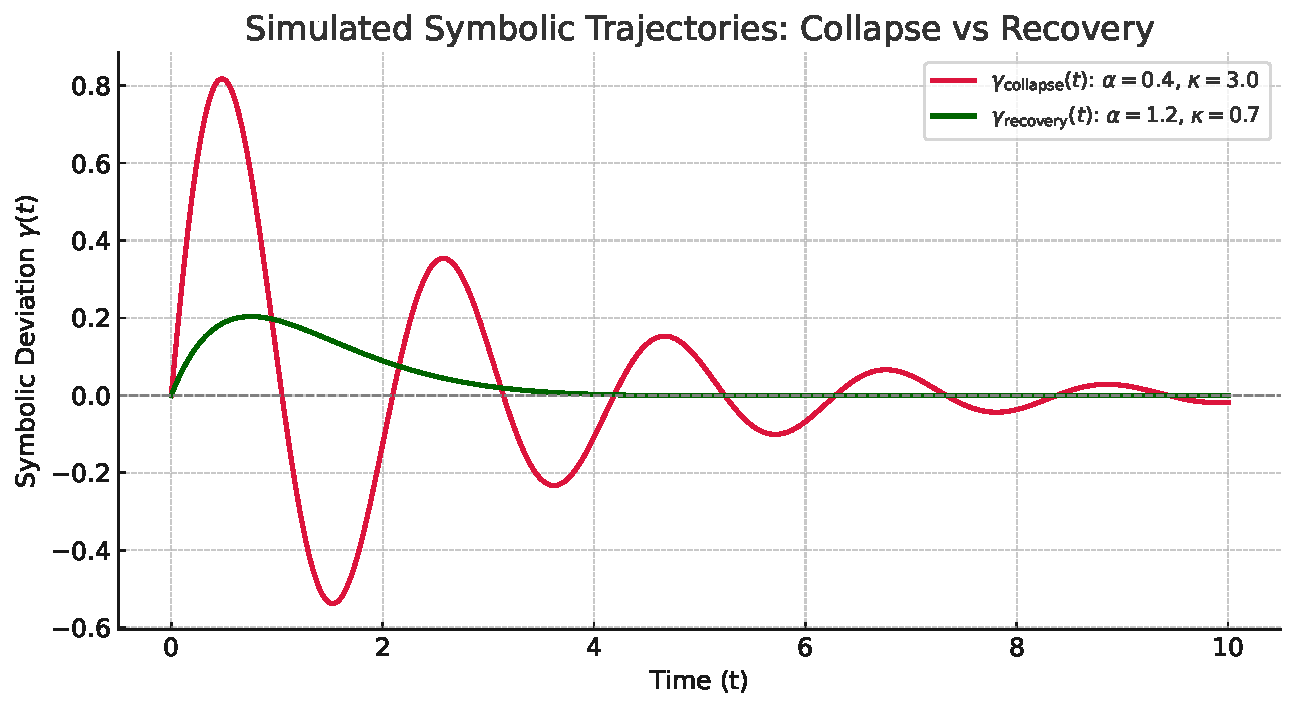
\includegraphics[width=0.9\textwidth]{figs/simulated_gamma_trajectories.pdf}
  \caption{Simulated symbolic deviation $\gamma(t)$ under two epistemic configurations. The collapse profile (red) exhibits disorganized, unstable behavior. The recovery profile (green) shows coherent symbolic re-anchoring.}
  \label{fig:gamma_simulation}
\end{figure}

These simulations help visualize how symbolic systems evolve in time depending on their semantic curvature and memory. The method suggests that symbolic collapse and recovery could be quantitatively modeled in clinical narratives and linguistic data using time-dependent entropic metrics and phase space flows.

This model also opens the path for future extensions with stochastic noise, attractor detection, and dynamic bifurcation mapping across individual narrative profiles.


\subsection*{5.7 Pseudocode for Symbolic Simulation}

To foster reproducibility and enable integration into clinical-symbolic instrumentation, we include a simplified Python pseudocode representing the simulation of symbolic deviation $\gamma(t)$ under different parameter regimes:

\begin{lstlisting}[language=Python, caption={Simulation of $\gamma(t)$ for symbolic collapse and recovery}, label={lst:gamma_simulation}]
import numpy as np
import matplotlib.pyplot as plt

# Time vector
t = np.linspace(0, 10, 500)

# Profile 1 — Collapse: low anchoring, high curvature
alpha_1, kappa_1 = 0.4, 3.0
gamma1 = np.exp(-alpha_1 * t) * np.sin(kappa_1 * t)

# Profile 2 — Recovery: strong anchoring, mild curvature
alpha_2, kappa_2 = 1.2, 0.7
gamma2 = np.exp(-alpha_2 * t) * np.sin(kappa_2 * t)

# Plot both symbolic trajectories
plt.plot(t, gamma1, label="Collapse", color="red")
plt.plot(t, gamma2, label="Recovery", color="green")
plt.xlabel("Time (t)")
plt.ylabel("Symbolic Deviation γ(t)")
plt.title("Simulated γ(t): Collapse vs Recovery")
plt.legend()
plt.grid(True)
plt.show()
\end{lstlisting}

This pseudocode illustrates the symbolic differential decay of anchoring and the oscillatory behavior of curvature in the symbolic manifold. It can be extended to model real narrative data using NLP-derived time series and mapped into $(\alpha, \kappa, \mathcal{E}_r)$ coordinates.

\subsection*{5.6 Conclusion — Toward a Symbolic Clinical Geometry}

This module consolidates a translational geometry of mind—mapping symbolic cognition into a formal manifold $(\alpha, \kappa, \mathcal{E}_r)$ and interpreting clinical states as topological trajectories. Through this lens, collapse is not a failure but a bifurcation; recovery is not reversal but epistemic phase transition.

By integrating concepts from psychiatry, dynamical systems, pharmacology, narrative theory, and symbolic topology, we have outlined a new diagnostic paradigm: not one that reduces experience to symptoms, but one that reconstructs symptoms as vectorial flows in symbolic space. Clinical states emerge as differential geometries of meaning, and interventions—whether pharmacological, narrative, or computational—function as curvature-shaping operations.

Simulated archetypes, phase vector fields, and anchoring dynamics now serve not only as metaphors but as formalisms. They permit the modeling, anticipation, and symbolic engineering of cognitive states. This opens the door to symbolic instrumentation, personalized phase diagnostics, and real-time topological navigation of mental space.

Ultimately, symbolic medicine reframes care not as containment, but as transfiguration. The symbolic manifold becomes both map and mirror—reflecting a patient’s recursive topology while guiding their narrative reassembly across epistemic thresholds. This approach offers not a single solution, but a cartography for human complexity.
